
\section{Semisupervised Learning}
According to \citet{mohri2018foundations}, Semisupervised Learning is defined by:
\blockquote{The learner receives a training sample consisting of both labeled and unlabeled data,
  and makes predictions for all unseen points. Semisupervised learning is common in settings where
  unlabeled data is easily
  accessible but labels are expensive to obtain. Various types of problems arising
  in applications, including classification, regression, or ranking tasks, can be framed
  as instances of
  semi-supervised learning.}

This category is less common in Machine Learning than Unsupervised or Supervised learning.
For the case of Optimal Transport applications,
although Reinforcement Learning is a popular
branch of Machine Learning, not many works were obtained.
Transfer Learning was the only subcategory with a significant amount of work to be revised. 

\subsection{Transfer Learning}

Transfer Learning consists in adapting the knowledge gained from one domain to another. The
domain where labeled data is available is called source domain, and the transfer of knowledge is done
to a target domain. We can formally define it as the following:

\begin{definition}{(Transfer Learning)}

Let
$\mathcal D_s = \{\mathcal X_s, P_s(x_s)\}$ and
$\mathcal T_s = \{\mathcal Y_s, P_s(y_s \mid x_s)\}$
define the domain source and task source, and 
$\mathcal D_t = \{\mathcal X_t, P_t(x_t)\}$ and
$\mathcal T_t = \{\mathcal Y_t, P_t(y_t x_t)\}$
define the domain target and task target.
Then Transfer Learning aims to improve the learning of the
target predictive function $P_t(y_t \mid x_t)$, using knowledge gained
from the source, where $(\mathcal D_s, \mathcal T_s) \neq (\mathcal D_t, \mathcal T_s)$.
\end{definition}

The field of Transfer Learning can be split in many subcategories according to the assumptions
made on the domain and tasks of both source and target.
The most studied subcategory is Domain Adaptation, where the source and
target are assumed to share the same task, but have different marginal distributions on the data.
In the Appendix \ref{sec:transferlearning}, we expand on the different ways Transfer Learning
is usually categorized.

Besides the different types of Transfer Learning problems,
there are also a vast number of methods for transferring knowledge. For example,
sharing the model parameters, using re-weighting
schemes to account for the difference in data distribution or
finding a similar subspace where both source and target domains can be represented.

\vspace{5mm}
\noindent \textbf{Optimal Transport for Label Propagation in Graphs}
\vspace{3mm}

To our knowledge, \citet{solomon2014wasserstein} was the first to use OT for semi-supervised learning.
The authors tackled the problem known as label propagation in graphs.
Suppose that only a portion of the vertices have known information, and this information consists in
a distribution. The goal is to predict the distribution in the vertices of the graph where
there is no information. This type problem is very common in Transfer Learning. Take for example traffic prediction,
where one has the traffic distribution of 24-hours in some intersections, and the goal is to
somehow predict the distribution in the intersections where there is no information. Other example is
weather forcasting, where information there is information only in a subset of cities, and we wish to predict
this information for where there is no data.

The model proposed by \citet{solomon2014wasserstein} consisted in using the 2-Wasserstein distance to
propagate the distributions across the vertices, where the weight in the edges symbolized the geometric distance.
Given two distributions $\mu$ and $\nu$ in two vertices, and a vertice in the middle with unknown information.
The model proposed by \citet{solomon2014wasserstein} seeks to minimize the Dirichlet energy, in which the
Wasserstein distance is used to measure the discrepancy between the distributions:
\begin{equation}
  \mathcal{E}_D[f]:= \sum_{(v,w)\in E} \omega_e W_2(\mu_v, \mu_w),
\end{equation}
where $E$ is the set of edges, $v$ and $w$ are two vertices connected by an edge, $\omega_e$ is the weight
of the edge, $\mu_v$ and $\mu_w$ are the distributions on each vertex.


\vspace{5mm}
\noindent \textbf{Optimal Transport Domain Adaptation}
\vspace{3mm}

Similar to the work of \citet{arjovsky2017wasserstein}, the work of \citet{courty2014domain}
is seminal in the use of Optimal Transport for Machine Learning. From it, many
other works have been developed, either extending it or proposing new methods base
on the main idea introduced in the paper.

\citet{courty2014domain} proposed to use OT to tackle the problem of Unsupervised Domain Adaptation,
that corresponds to the case where there is no label at all in the target.
The authors assume that the difference in the source and target distribution is due to an
unknown transformation $T:\mathcal X_s \to \mathcal X_t$, but that this transformation
still preserves the conditional distribution:
\begin{equation}
  P_s(y \mid x^{s}) = P_t(y \mid T(x^{s})).
\end{equation}
The main idea behind the model, which we call OTDA, consists in finding an Optimal Transport map
from the source data distribution
$\mu_s = \sum^{n_s}_{i=1}u_i^{s} \delta_{x^s_i}$ to the target data distribution
$\mu_t = \sum^{n_t}_{i=1}u_i^{t} \delta_{x^t_i}$. Then, use it to transport the source data
to the target data. After this, the model trained on the transported source data can
be immediately used on the target data. This process is illustrated in Figure \ref{fig:otda}.

\begin{figure}[H]
  \centering
  \def\svgscale{0.8}
  \includesvg[inkscapelatex=false]{Figures/otda.svg}
	\caption{Schematic drawing of the OTDA algorithm. $T$ corresponds to the unknown transformation
  between the source and the target.
  The shape of the markers represent the class label of each data sample, and the color indicates from which dataset
  they belong (blue for source and red for target). The line in green represents the learned classifier.}
	\label{fig:otda}
\end{figure}

To find an Optimal Transport map, one would need to solve the Monge Problem, which would be quite computationally
expensive. Instead, \citet{courty2014domain} suggest to solve the Kantorovich Problem with Entropic Regularization,
thus, using the Sinkhorn algorithm to find the Optimal Transport plan.
One cannot use the transport plan to transport the source data,
since the transport plan may split the sample data. Instead, the authors propose the use of \textbf{barycentric mapping},
which is
\begin{equation}
  \hat{x^s_i} = \mathrm{argmin}_x \sum_j \bm \gamma^*(i,j) c(x,x_j^t),
  \label{eq:barycentricmapping}
\end{equation}
where $\gamma^*$ is the OT plan with entropic regularization. Note that if the cost function
is the squared $L_2$ distance, then this mapping is just the weighted average. The barycentric
mapping is illustrated in Figure \ref{fig:barycentriccoordinate}.

\begin{figure}[H]
  \centering
  \def\svgscale{0.8}
  \includesvg[inkscapelatex=false]{Figures/barycentriccoordinate.svg}
	\caption{Example of barycentric coordinate mapping if the cost function is the squared $L^2$ distance in
  $\mathbb R^2$. The circle in blue represents one data sample from the source, the circles in red
  represent the target data, the circle in blue with dotted line represents the barycentric mapping
  of the source sample, and the lines in gray represent the optimal transport plan.}
	\label{fig:barycentriccoordinate}
\end{figure}

\citet{courty2014domain} also proposed the addition of an extra regularization term to the
Entropic OT problem in order to enforce transport only inside the same class label.
The idea is to avoid transport plans where, for example, a data sample $x_j^t$
receives the same amount of mass from samples $x_i^s$ and $x_k^s$, where sample $i$ has
a class label different than sample $k$. Therefore, the OT problem becomes:
\begin{equation}
  \gamma^* = \underset{\gamma \in \Pi(\mu_s,\mu_t)}{\mathrm{argmin}} \overline{OT}_{c,\varepsilon}(\mu_s,\mu_t)
  + \eta \sum_j \sum_l || \bm \gamma(\mathcal I_l, j)||^p_q,
  \label{eq:otda}
\end{equation}
where $\eta >0$, $\mathcal I_l$ is the set of indices of samples with class label $l$, and
$\bm \gamma(\mathcal I_l, j)$ is a vector containing the coefficients of the $j$th column
of the transport plan matrix $\bm \gamma$ associated to class $l$.

\citet{courty2014domain} used $p=1/2$ and $q=1$ for algorithmic reasons.
In a follow up paper, \citet{courty2016optimal} suggested using
$p=1$ and $q=2$, also known as group-lasso regularizer,
and devised an efficient algorithm for solving \eqref{eq:otda}.
The authors also proposed to use Laplacian regularization, but the experimental
results comparing the three types of regularization
showed that the group-lasso outperformed the others.

\citet{rousselle2015optimal} proposed two new algorithms
for the case where there is some known labels in the target data. In both algorithms the target data with known labels ($X_{k}$)
is transported to the target data with unknown label ($X_{u}$) using the OT formulation from
\citet{courty2014domain}. The first algorithm consisted in
splitting the data according to class label, and then finding an OT plan for couple $(X_{s}^l, X_k^l)$,
where $X_s^l$ is the portion of the source dataset with label $l$, and $X_k^l$ is the portion of the target
dataset with known label $l$.
The second algorithm consisted in finding a plan between $X_{s}$ to $X_{k}$
without caring for the classes, and then performing a post processing on the optimal transport plan matrix
$\mathbf \gamma$ such that each entry of the matrix with class-crossing is sent to zero, and the matrix is renormalized.

% \citet{alvarez2018structured} proposed a sub-modular regularization that enforces structures in
% the Optimal Transport matrix at the same time these structures are estimated. Hence, this could
% be used to perform the mapping between source and target.

\vspace{5mm}
\noindent \textbf{Joint Distribution Domain Adaptation}
\vspace{3mm}

The OTDA algorithm assumed that the labels were transported along the features,
which might not always be true.
\citet{courty17jdot} devised the model named Joint Distribution Domain Adaptation (JDOT),
where such restriction was relaxed.
The main idea of the model is to align the feature/label space of the source and target,
at the same time the classifier $f$ is learned.
% In the case that no label is present in the target, the authors proposed the use of
% $f(x_t)$ to satisfy the role of $y_t$, where $f$ is the classifier the model seeks to estimate.

The JDOT algorithm seeks to solve the following optimization problem:
\begin{align}
  \nonumber
  &\min_{f \in H} OT_c(\hat{\mathcal P}_s, \hat{\mathcal P}_{t,f}) \\
  &\mathrm{s.t.} \quad 
  c((\mathbf x_1,y_1),(\mathbf x_2, y_2)) = \alpha ||\mathbf x_1 - \mathbf x_2||^2 + \mathcal L(y_1,y_2),
  \label{eq:jdot}
\end{align}
where $\alpha >0$, $\mathcal L(y_1,y_2)$ is the loss function for a classification task,
$\hat{\mathcal P}_s$ is the empirical distribution of $(X_s,Y_s)$ and
$\hat{\mathcal P}_{t,f}$ is the distribution of $(X_t, f(X_t))$. Note that since the target is unlabeled,
we use the learned classifier to come up with the labels.

Problem \eqref{eq:jdot} can be optimized in an alternative way. First, fixing $f$,
we have to solve an Optimal Transport problem, which can be done using Linear Programming
algorithms such as the Simplex, or, we can regularize the problem and solve with
the Sinkhorn algorithm. Then, for a fixed transport plan $\gamma^*$, we minimize $f$.
\citet{courty17jdot} suggested the use of either Block Gradient Descent or Gauss-Sidel method.
The authors showed that the JDOT method outperformed many state-of-the-art Transfer Learning
algorithms, including OTDA.

\citet{damodaran2018deepjdot} expanded the JDOT model with their DeepJDOT, which uses Deep Neural Networks
to learn a representation $g$ of the data at the same time it learns the classifier $f$. The new optimization
problem then becomes
\begin{align}
  \nonumber
  \min_{\mathbf P \in \mathcal P, f,g} \frac{1}{n^{(s)}} \sum_i \mathcal L_s(y_{i}^{(s)}, f(g(x_i^{(s)})))
  + \sum_{i,j} & \mathbf P_{i,j} (\alpha |g(x_i^{(s)}) - g(x_j^{(t)})|^2 \\ &+
  \lambda_t \mathcal L_t (y_i^{(s)}, f(g(x_j^{(t)}))),
\end{align}
where $\mathcal L_s$ and $\mathcal L_t$ are the loss functions used in the source and target respectively.
The authors proposed to solve this minimization problem with stochastic approximations
using gradient descent in both the source and target.
Experimental results showed that DeepJDOT consistently outperformed the other Deep Learning methods to which
it was compared, such as DeepCORAL \citep{sun2016deep}.

\begin{figure}[H]
	\centering
	\includegraphics[width=12cm]{Figures/deepjdot.png}
	\caption{Figure from \citet{damodaran2018deepjdot} illustrating the DeepJDOT model.}
	\label{fig:geometricdataset}
\end{figure}

Another model based on JDOT was proposed by \citet{redko2019optimal}. While JDOT focuses on covariate
shift (Figure \ref{fig:covariateshift}), the model proposed by \citet{redko2019optimal},
called Joint Class Proportion and Optimal Transport
(JCPOT), focuses on the problem of target shift (Figure \ref{fig:priorshift})\footnote{Target shift
is also known as prior shift.}. The main idea of the model is to
reweigh samples in the source to compensate the discrepancy in class proportion between the sources and the target.
Both the Optimal Transport plans and the class proportion in the target are estimated jointly by solving a
constrained Entropic Wasserstein Barycenter problem.

Let $\mu^{t}$ be the empirical distribution
of the target dataset, to which we don't know the label, $\mu_1^{s},...,\mu_k^{s}$ the empirical
distribution for the sources to which we do know the label, and $n^s_{i}$
the number of samples in each source data. For each source, define $\mathbf h_i$ to
be the vector containing the proportion of each class, and $\mathbf D_{h_i}$ a linear transformation
such that $\mathbf D_{h_i} \mathbf h_i = [\frac{1}{n^s_i},...,\frac{1}{n^s_i}]^\mathrm T$ which is the vector
of equal weights of the empirical distribution $\mu^{s}_i$\footnote{Remember that
$\mu^{s}_i = \frac{1}{n^s_i}\sum^{n^s_i}_j \delta_{x_j^s}$, where each sample has equal weight.}.
This allows us to write the source distribution as a function of the proportions of each label as
$\mu_s = (\mathbf D_{i} \mathbf h_i) \bm \delta_{\mathbf X_i}$.
Thus, the optimization for the Barycenter problem for JCPOT becomes
\begin{equation}
  \underset{\mathbf h \in \Delta^l}{\mathrm{argmin}} \sum^k_{j=1}
  \lambda_j W_{1,\varepsilon} \left( 
  (\mathbf D_{i} \mathbf h_i) \bm \delta_{\mathbf X_i}, \mu^{t}
    \right),
    \label{eq:jcpot}
\end{equation}
where $\Delta^l := \{\alpha \in \mathbb R^l_+ \ : \ \sum^l_{i=1} \alpha_i = 1\}$ and $l$ is the number of classes.
Solving \eqref{eq:jcpot} gives an estimate on the class proportions of the target, and one can
reconstruct the sources distributions as $\mu^s_i = (\mathbf D_{i} \mathbf h^*)$ wher $h^*$
is the argument that minimizes \eqref{eq:jcpot}. The next step is to find the Entropic OT plan
from each $\mu^s_i$ to $\mu$.
The labels in the target are estimated by calculating the proportion of mass coming from each label
in the source, akin to a
boosting technique. Figure \ref{fig:jcpot} compares the JCPOT with OTDA by \citet{courty2014domain}, which
does not take into account the target shift.

\citet{turrisi2020multi} uses the same modified Wasserstein distance as JDOT, but apply it instead
to the case of multiple sources. The authors propose to weight each source according to its proximity
to the target. The optimization problem proposed is
\begin{equation}
  \min_{\mathbf \alpha \in \delta^S , f} W_{JDOT}\left(\hat{p}^f,
      \sum^S_{s=1} \alpha_s \hat{p}_s
  \right),
\end{equation}
where $S$ is the number of sources and $\delta^S$ is the simplex of dimension $S$.

\begin{figure}[H]
	\centering
	\includegraphics[width=14cm]{Figures/jcpot.png}
	\caption{Figure from \citet{redko2019optimal} illustrating the importance of
  proportion estimation for target shift: (a) 2 sources and 1
target with different class proportions; (b) Transport plan from OTDA \citep{courty2014domain};
(c) Transport plan using OTDA with reweigh based on true class proportions;
(d) Transport plan obtained with JCPOT without knowing the true class proportion.}
	\label{fig:jcpot}
\end{figure}

Transport plans obtained from the solution of discrete OT problems cannot be used for out-of-sample
data, since they are matrices transporting each data point on which the model was trained. The work
of \citet{perrot2016mapping} is perhaps the first to address this issue by proposing a method
to estimate the underlying transport map $T$ that approximates the learned optimal transport plan.
The authors propose a joint optimization problem, where one seeks to
learn a transformation $T$ regularized by a transport plan. The optimization problem is
\begin{equation}
  \underset{T \in \mathcal H, \gamma \in \Pi(\mu_s,\mu_t)}{\mathrm{argmin}}
  \frac{1}{n^{(s)} d_t} ||T(\mathbf X^{(s)}) - n^{(s)} \gamma \mathbf X^{(t)}||^2 +
  \frac{\lambda_\gamma}{\max(\mathbf C)}\langle \gamma, \mathbf C\rangle +
  \frac{\lambda_T}{d_s d_t} R(T),
\end{equation}
where $d_s, d_t$ are the dimensions of the source and target, $\lambda_s$ and $\lambda_t$ are hyper-parameters,
$R(\cdot)$ is a generic regularization term.
For the space $\mathcal H$ of possible transport maps, the authors experimented with the space of linear maps,
and the space of non-linear maps using the kernel trick.

\vspace{5mm}
\noindent \textbf{Geometric Dataset Distance}
\vspace{3mm}

Models such as JDOT assume that the label set from the source and the target are the exact same, but this
is not always true. For example, one might want to transfer knowledge from a model trained on the MNIST
dataset to perform handwritten digits recognition, to instead perform handwritten letters recognition.
The work of \citet{alvarez2020geometric} proposes a very elegant way of measuring the distance between
dataset (i.e. features and labels). This new metric is a hierarchical Optimal Transport distance,
because it uses an OT metric inside another OT metric. The authors named this new metric as Optimal
Transport Dataset Distance (OTDD) and is given by
\begin{equation}
  d_z((x,y),(x',y')):= (d_x(x,x')^p + W_p(\alpha_y,\alpha_{y'}))^{1/p},
\end{equation}
where $x$ is a sample in the feature set, $y$ is a sample from the label set, $d_x$ is a metric defined
in the feature space, and $\alpha_y(x) := P(X = x \mid Y = y)$ is the conditional distribution of
obtaining a sample $x$ given a label $y$. Note that to calculate $d_z$ one needs to solve an OT problem
inside another OT problem, thus becoming quite computationally expensive. \citet{alvarez2020geometric}
proposed different methods for dealing with such computational complexity, such as using the
Sinkhorn divergence, and considering $\alpha_y$ to be Gaussian which leads to a closed form solution.
Then, the authors showed how OTDD correlated with transferability capacity of different datasets,
such that it could be used as criterion for source dataset selection to perform transfer learning.
Figure \ref{fig:geometricdataset} exemplifies the capacity of OTDD to the use of label-agnostic OT distance.

\begin{figure}[H]
	\centering
	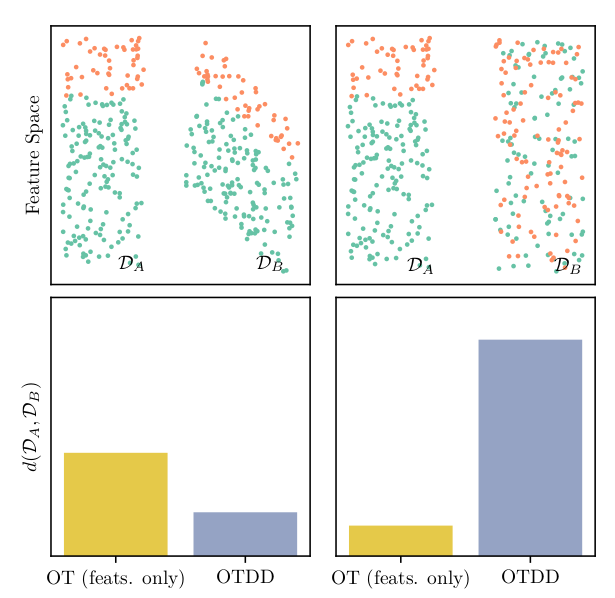
\includegraphics[width=7cm]{Figures/geometricdataset.png}
	\caption{Figure from \citet{alvarez2020geometric} illustrating the OTDD distance.}
	\label{fig:geometricdataset}
\end{figure}

\vspace{5mm}
\noindent \textbf{Transfer Learning with Adversarial Networks}
\vspace{3mm}

In Transfer Learning, there are many methods that use adversarial learning to train a discriminator
to distinguish source and target, while a generator tries to learn a representation of the data.
\citet{lee2019sliced} proposed the use of Sliced-Wasserstein distance with the task-specific adversarial
learning model, introduced by \citet{saito2018maximum}. They named their model Sliced-Wasserstein Discrepancy (SWD).

The model consists of a generator and two discriminators that are initialized with different weights.
Hence, the model produces two different decision boundaries. The training then consists of freezing the parameters
of the generator, and
maximizing the
discrepancy between the decision boundaries while keeping the classification accuracy of each discriminator. Then,
freezing the discriminators, and training the generator to minimize the discrepancy.
\citet{lee2019sliced} contribution consists in using the Sliced-Wasserstein distance to measure such discrepancy.
The method is summarized in Figure \ref{fig:swd-tl}.


\begin{figure}[H]
	\centering
	\includegraphics[width=14cm]{Figures/mcd-transfer-learning.png}
	\caption{Figure from \citet{saito2018maximum} illustrating the task-specfic adversarial learning algorihtm.}.
	\label{fig:swd-tl}
\end{figure}

\vspace{5mm}
\noindent \textbf{Model Ensemble and Feature Selection}
\vspace{3mm}

\citet{shen2018wasserstein} used a Neural Network with structure similar to WGAN, where a discriminator
was used to estimate the Wasserstein distance between the source and target samples, while
another network optimizes a feature extractor. This model was named
Wasserstein Distance Guided Representation Learning (WDGRL).


Another very unique approach was proposed by \citet{sidakfusion20}, where it was proposed
a method of ensembling neural networks, which successfully yielded ``one-shot'' knowledge transfer.
The method consisted in using the Wasserstein barycenter as a way of averaging the
weights in the neural networks, performing Optimal Transport layer by layer.
% In order to solve an Optimal Transport problem between the network's layers,
% one needs to define a ground cost. The authors propose two different strategies
% for this: a first one consists in using the incoming weights of the incoming 

Similarly to \citet{sidakfusion20}, the work of \citet{li2020representation} also uses OT on a
Neural Network architecture, but instead of finding a barycenter for model parameters, this work
proposes to use the discrepancy in the source network and the target network as a regularizer
when training the target network. Again, the use of OT comes to metrize the discrepancy in the networks.
Figure \ref{fig:rtlot} sketches how the algorithm works.

\begin{figure}[H]
	\centering
	\includegraphics[width=11cm]{Figures/rtlot.png}
	\caption{Figure from \citet{li2020representation} illustrates the process of training the target Neural Network
  by adding the regularization term based on the discrepancy with the parameters of the source Network. In the image,
  $\mathbf M$ is the transport cost matrix, $\mathbf P$ is the optimal transport plan matrix, and $\Omega_P$
  represents the regularization term.}
	\label{fig:rtlot}
\end{figure}

\citet{gautheron2018feature} proposed to use Entropic OT for feature selection for unsupervised
Domain Adaptation. The authors argue that every dataset is composed of cartesian product
of a feature space $\mathcal F$ (i.e. column space) and an instance space (i.e. row space).
The main idea consists in finding an Optimal Transport plan $\gamma^\mathcal F$ from the
feature space of the source to the feature space of the target, such that the $k$ features with
higher transport rate from and to itself, i.e. $\gamma^\mathcal F_{i,i}$ are selected.
Since the number of rows is usually different between source and target, a sampling
method is proposed in order to select rows such that both end up with the same size, thus
enabling the use of OT, where each feature (column) is a point mass $\delta_{f_i}$ with dimension
equal to the number of rows.

% \citet{lee19hier} proposed the use of Hierarchical Optimal Transport for dataset alignment
% between source and target when the data presents a clustered structure, that is, when
% the data is multi-modal such as in Gaussian Mixtures. The model, named
% \textit{Hierarchical Wasserstein Alignment} (HiWA), seeks to jointly learn a transformation
% $T$ and the cluster correspondence. The key insight from the authors is that the hierarchical
% structure decomposes the optimization surface in simpler ones, reducing the chances
% reaching a local minima.

\vspace{5mm}
\noindent \textbf{Transfer Learning Across Incomparable Spaces}
\vspace{3mm}

The work of \citet{yan2018semi} tackled the problem of Heterogeneous Domain Adaptation (HDA), in which the space
of the source and the target is different (e.g. source is in $\mathbb R^3$ and target is in $\mathbb R^2$).
Due to the differing spaces, the authors use the entropic Gromov-Wasserstein metric (EGW) to find the optimal transport
between the source and the target.
Their method, called Semi-supervised Gromov-Wasserstein (SGW), is similar to OTDA proposed by \citet{courty2014domain},
and it also works by transporting the source to the target and then performing the training.